% This template was originally by R. Jacob Vogelstein
% Updated on March 1, 2010 by Noah J. Cowan


\documentclass[12pt,oneside,final]{thesis}

\usepackage[superscript]{cite}
\usepackage{amsmath,amsfonts}
\usepackage{graphicx}
\graphicspath{{./figs/}}
\usepackage{fixltx2e}
\usepackage{array}
% wrapfig is fragile: use sparingly
\usepackage{wrapfig} 
%\usepackage{times}  % Use this for ugly fonts

\usepackage{upgreek}
\usepackage{hyperref}
\usepackage{setspace}

\usepackage{booktabs}
\usepackage{multirow}
\usepackage{longtable}
\usepackage[font=singlespacing, labelfont=bf]{caption}
%\usepackage{CV}

\usepackage{enumitem}
\newlist{inlinelist}{enumerate*}{1}
\setlist*[inlinelist,1]{%
  label=(\arabic*),
}

\usepackage{fancyhdr}    % Use nice looking headers along with the required footer page numbers   
%\usepackage[hypertex]{hyperref}

%Define the header/footer style
\pagestyle{fancy}
\fancyhf{}
\setlength{\headheight}{15pt}
\lhead{\leftmark}
\cfoot{\thepage}
\renewcommand{\headrulewidth}{0pt}
\fancypagestyle{plain}{% Redefine ``plain'' style for chapter boundaries
\fancyhf{} % clear all header and footer fields
\fancyfoot[C]{\thepage} % except the center
\renewcommand{\headrulewidth}{0pt}
\renewcommand{\footrulewidth}{0pt}}

%\tolerance=10000

%\makeglossary % enable the glossary

\begin{document}

\title{Thesis Proposal : Modulo7 : A full stack Music Information Retrieval and Querying Engine using Music Theoretic Principles}
\author{Arunav Sanyal}
\degreemonth{December}
\degreeyear{2015} 
\thesis
\masterscience
\copyrightnotice


% add your chapters, best way is to have separate TeX files for each chapter
%% FRONTMATTER
\begin{frontmatter}

% generate title
\maketitle

\begin{abstract}

\noindent Music Information Retrieval (MIR) is an interdisciplinary science of extracting non trivial information and statistics from music data sources. In today's digital age, music is stored in a variety of digitized formats - e.g midi, musicxml, mp3, digitized sheet music etc. Music Information Retrieval Software aim at extracting features from one or more of these source. MIR research helps in solving problems like automatic music classification, recommendation engine design etc. Users can then query the acquired statistics to acquire relevant information. \\\\
The author proposes and implements a new Music Information Retrieval and Query Engine called Modulo7. Unlike other MIR software which deal with low level audio features, Modulo7 operates on the principles of music theory and a symbolic representation of music. Modulo7 is a full stack deployment, with server components that parse various sources of music data into its own efficient internal representation and a client component that allows consumers to query the system with sql like queries which satisfies certain music theory criteria (and as a consequence Modulo7 has a custom relational algebra with its basic building blocks based on music theory). 

\vspace{1cm}

\noindent Primary Reader: Dr David Yarowsky\\
Secondary Reader: Dr Yanif Ahmad

\end{abstract}

\begin{acknowledgment}

I would like to thank Dr David Yarowsky for giving me the opportunity to work on this project. His detailed insights have immensely helpful to me to power through my work. I would like to thank Dr Yanif Ahmad for his crucial help in the systems aspects of my query engine and the implementation of the server side components. 

\end{acknowledgment}

\begin{dedication}
 
This thesis is dedicated to my family and to all the music lovers in the world. 

\end{dedication}

% generate table of contents
\tableofcontents

\end{frontmatter}

\chapter{Introduction}
\label{sec:intro}

\noindent Why does a person like a particular song? What are the inherent aspects of a song that pleases a person's musical taste? Is it the complexity of a song, the beat the song or just a particular melodic pattern ? More so if a person likes a song, can we predict if he/she will like a similar song? If so then how is this similarity judged? \\\\
Music has been created since the dawn of civilization and these questions have plagued mankind just as long. In response to this, man has created elaborate systems of formal study for music and classification techniques in almost every ethnic community since antiquity. Two notable examples are the western system of solfege and classical music theory and the Indian system of raagas. These elaborate systems are based on very simple fundamental building blocks of melody and harmony and simple rules that govern the interplay of these building blocks. However very complex pieces of music can be created with these simple rules depending on the skill and virtuosity of artists. Composers use these rules and concepts to create novel music for mass consumption. \\\\
In the modern era industry and academia have attempted to address the problem of music recommendation and music classification. Industry has predominantly favored approaches that look at user preferences and history. For example Amazon Music recommendation works on consumer behavior (user's shopping, browsing history and related consumer behavior \cite{amazonreco}). Pandora on the other hand utilizes musicologists to ascertain how a song is similar to another song and creates software that leverages this ad-hoc generated data \cite{musicgenomepandora}. These approaches are either expensive in the human labor needed or in the amount of data processed that is input from a large number of users. More recently, companies like Echo Nest have extensively extracted features from music sources \cite{echonestfingerprint} and mined cultural information on the web but leave it for the consumers to determine how best to leverage this extracted data. Hence symbolic MIR is not traditionally used in industry and music theory is an after thought in almost all industry applications. \\\\
Academia on the other hand attempts to solve very particular problems in MIR. Typical examples would be cover song detection, processing information via signal processing, audio feature extraction, optical music recognition etc. In most cases the applications are of a very specific domain and does not fully scale with bulk music data. Generic frameworks like the jMIR \cite{jMIR} (which also happens to be a major inspiration for Modulo7) suite for automatic music classification exists, which is meant to facilitate research in MIR with a machine learning focus. However academia is disconnected with industry and no full scale MIR engines can satisfy the scale of industry applications. \\\\
This work is attempt to bridge both communities. Modulo7 is a full stack deployment of Music Information Retrieval Software, providing both a server architecture and a sql like client to query based on music theory criteria. Modulo7 does not attempt to solve very complex music theoretic problems (e.g study orchestral music to identify counter point class). Rather Modulo7 acts a framework on which such analysis can be built upon. Most importantly, Modulo7 addresses the issue of scale and allows a fast comparison between songs on certain music theoretic criteria. It also addresses deficiencies in existing software, such as filling up incomplete meta data information in music sources. Certain problem statement of this sort would be Key estimation, Tempo estimation etc. \\\\
Modulo7 implements a unique indexing scheme and a universal "document" representation of music. This indexing scheme involves creating an inverted index for global properties of songs (key signature, the property of homophony, time signature etc). This indexing scheme allows for fast lookups for certain types of queries (e.g find all songs that in the key of C Major) and also allows for speedup in scenarios which require criteria based on indexed terms. 
\chapter{Software architecture and Methodology}
The following sections present the software architecture of Modulo7.
\section{Server Side architecture}
\noindent Modulo7 is designed with the purpose of scalability. A block diagram of the components of the server side architecture is presented below :-
\begin{enumerate}
\item Source Converter : Converts music sources (e.g. music XML, midi etc) into modulo7's binary representation.
\item Music Theory Models : The model is a description of music theoretic criteria that can be applied on top of a song. Examples would be melodic contour, tonal histogram etc. 
\item Distributed Storage Mechanism : The modulo7 internal representation is a conversion to create a song representation with all the meta data of the song (Key, Scale,  etc) along with the sequences of note events stored as lists. This representation is then serialized and stored in and Hadoop Distributed File System. This allows for fault tolerance and a distributed deployment of the input data.
\item Lyrics Indexer : A distributed index of songs lyrics. This acts as a base on which standard techniques for similarity analysis might be applied. Alternatively it can provide a framework on which custom models (e.g. semantic intent of the song, correlation between music theory models and lyrics might also be applied).  
\item Lyrics similarity models : A set of similarity models that can be applied to an index. 
\item Query Engine : An SQL like interface to a client that allows you to gather and ascertain useful information (based on music theoretic criteria). 
\end{enumerate}

\begin{figure}
\centering
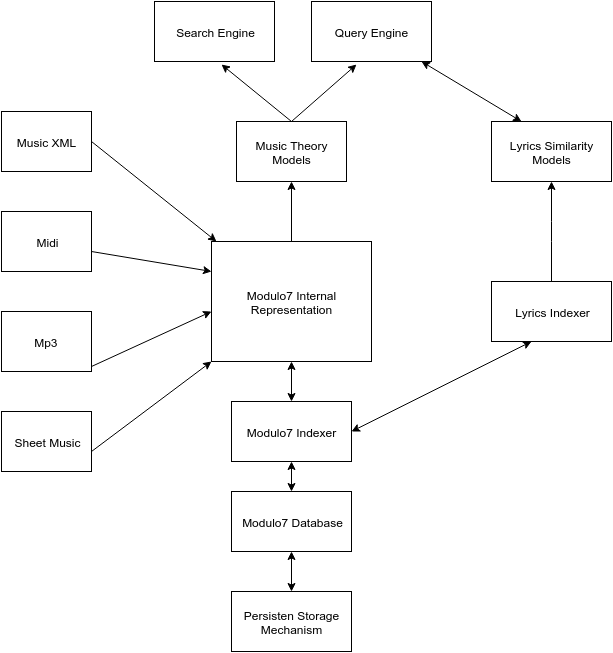
\includegraphics[width=\textwidth]{Modulo7Architecture.png}
\makeatletter
\let\@currsize\normalsize
\caption{Modulo7 architectural design}
\label{fig:figure}
\end{figure}
\newpage
\section{Client architecture}
\noindent The server exposes a sql like interface as well as a consumable API. Some sample queries would be :-
\begin{enumerate}
\item select midi files from database where $melodic\_complexity > some threshold$
\item select * from database where $artist = led\_zepplin \ and \ harmonic\_movement > harmonic\_movement(stairway\_to\_heaven)$
\item select $ num\_voices \ from \ Database \ where \ songName = someSong.midi$ 
\end{enumerate}

An API will also be exposed to the client along a remote invocation procedure. The API would primarily target single sources for specifics. Some example API would be :-
\begin{enumerate}
\item int getNumVoices(String midiFilePath)
\item double melodicContourMovement(String pngSheetFilePath)
\item double compareAverageAttack(String musicXMLFile)
\end{enumerate}

This API can be consumed for specific song analysis. As design this API will not work on a bulk of files like its sql counterpart. \\

Moreover the client also exposes a highly customized search engine based on the custom vector space representation of features extracted by Modulo7.

\section{Song sources}
\noindent At the heart of Modulo7's design is its song sources adaptors (or converters) into its own internal binary format. Each music source is a different representation and while certain sources ascribe what how music should be played (e.g musicxml, sheet music), other formats ascribe what is actually being played (e.g midi, mp3). There are many other music sources in existence (e.g guitar tablature, GUIDO format, humdrum format), but for the purposes of breadth and ubiquity, these four sources have been targeted as input for Modulo7. Note that acquiring features from each format is a domain specific challenge and inaccuracies are inherent because of that. The following subsections describe the individual formats in detail and the challenges encountered in parsing them.

\subsection{Midi format}
\noindent MIDI (short for Musical Instrument Digital Interface), is a technical specification for encoding of events on a midi enabled instrument and a protocol for interfacing and communicating between various midi enabled instruments. Typically any midi enabled electronic instrument when played, relays to its internal circuitry a message. Examples of such messages could be a particular note is being hit on a keyboard, a note is being hit off after being hit on, tempo based messages on the number of ticks per second etc. While MIDI is a technical specification for encoding music the score is being played, Modulo7 treats it as a symbolic representation of music. Midi was also a simple and popular encoding format for music and gaming industry in the nineteen ninties. \\\\
A symbolic representation is a codification of music which acts a higher level of abstraction (individual notes or chords being played) as compared to lower level representations like audio files (which codify information like waveforms). Modulo7's internal representation is also a symbolic representation. Symbolic representations are easier to manipulate when applying a music theoretic criteria. \\
Midi is one of the easier formats to parse for musical specifications. Moreover there is a big volunteer community of midi encoders. As such acquiring and parsing non trivial amounts of midi data is not a very challenging task. 

\subsection{Western Sheet Music}
Sheet music is one of the oldest forms of music in existence. Its a hand written or printed form of music that uses a specific script (a set of musical symbols on a manuscript paper) to ascribe music. Music Composers from Medieval and Modern periods of the western world use western sheet scripting to codify their work while performers play from these sources. A vast body of older work and particularly orchestral work is codified in sheet music. \\
Like midi, sheet music is also symbolic in nature. However unlike midi, its an expression of how a score should be played, rather than what is being played.  Modulo7 converts digitized versions of these sheet music (e.g sheet music stored .tiff, .png. jpeg etc formats)\\\\

A very simple example of sheet music for describing a melody is shown below. 

\begin{figure}
\centering
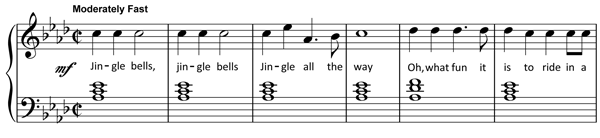
\includegraphics[width=\textwidth]{jingle-bells-sheet-music-piano.png}
\makeatletter
\let\@currsize\normalsize
\caption{Jingle bells melody sheet music representation	}
\label{fig:figure}
\end{figure}

Parsing digitized sheet music is an extremely challenging task. It requires a solid understanding on Computer Vision and even the state of the art software in existence today cant handle all scores (especially a poorly digitized formats). Given the amount of domain knowledge required, Modulo7 uses a third party library (insert TPL here). 

\subsection{Music XML format}
\noindent Music XML format is a standard open format for exchanging digital sheet music. A music XML format is unusual as its a format that is easy to parse for computers and easy for humans to understand it. MusicXML formats are heavily used by music notation applications. Music XML format is a symbolic format and can be considered a modernization of the Sheet music format. Its disadvantage however is unlike sheet music, a performer cant read the piece and play it on the spot directly. \\
Just like Western Sheet music and midi, music XML is a symbolic format as well. Music XML is also a transcription format which specifies how a score should be played. 

\subsection{MP3 format}
\noindent For the sake of completeness, Modulo7 also supports an audio format called mp3. Its an audio encoding format that uses lossy compression to encode audio data. Mp3 gives a reasonably good approximation to other digital audio formats of music storage with a significant savings in space for storage. Its one of the defacto standards of digital music compression and transfer and playback on most digital audio players. 

\section{Modulo7 Internal Representation}

\noindent Modulo7 consists of converters that convert data into Modulo7's internal representation. This representation can be thought of a document representation on which similarity measures described in Chapter 4 can be applied to. Moreover the internal representation can be thought of as an indexed meta data structure for any source of song from which relevant information can be acquired. Hence Modulo7 indexing schematic is a symbolic representation of music much like music xml and sheet music. The converters are responsible for converting different music sources to this representation format. Its important to note that depending on there source one or more of the subcomponents of the internal representation may be missing or wrong. Modulo7 indexes songs based on each of these criteria and on top of these boolean queries can be formulated. The components are broadly categorized as the following:-\\

\noindent \textbf{Song Metadata:} The metadata aspects in a song e.g. The name of the song/ the composer/performer's name, Key Signature of the Song, Meter of the Song etc. These are global properties of the song. \\

\noindent \textbf{Voices in a song:} Similar to the Voices in Music theory, Voices in Modulo7 represent the same symbolic data as is present in the sources from which the information is parsed.\\

\noindent \textbf{Lyrics of a song:} The textual representation (along with delimiters for line breaks) for the lyrics of a song. Lyrics can live independently as separate entities (if the input to Modulo7 is a text file containing the lyrics and no other information). However midi/musicxml and sheet music have optional lyrics elements present in their transcriptions and Modulo7 transcribes from those. \\\\
In most cases though lyrics exists as a separate entity from songs. In such cases, Modulo7 separately indexes lyrics. In certain datasets, the lyrics representation is different (for example the million song dataset has a representation format as a bag of words with counts of the words occuring for each format \cite{msd}). Modulo7 accomodates such formats as well.

\begin{figure}
\centering
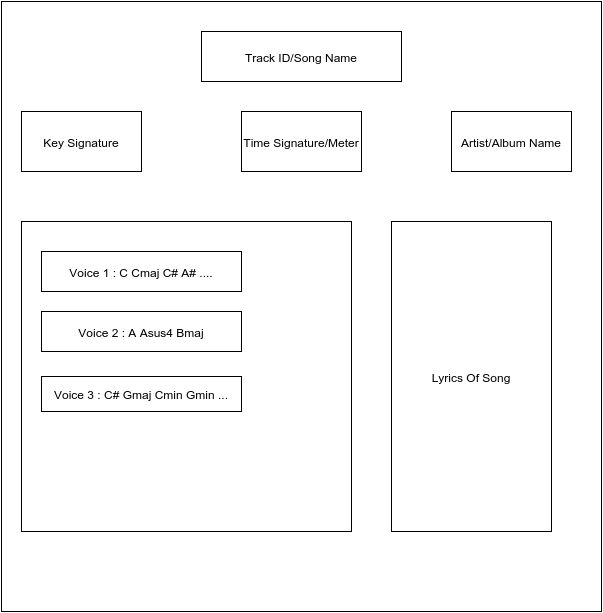
\includegraphics[width=\textwidth]{DocumentStructureOfModulo7.png}
\makeatletter
\let\@currsize\normalsize
\caption{Modulo7 internal representation}
\label{fig:figure}
\end{figure}

\section{Methodology}

\noindent This section contains the methodology followed in the information retrieval phase and then the indexing steps taken after the domain specific conversion is completed by Modulo7's adapters

\begin{enumerate}
\item Given a root directory, Modulo7 parses all the sheet music image files, mp3, midi and 
\end{enumerate}

\chapter{Progress Done}
The following points of progress have been successfully completed:-
\begin{enumerate}
\item Literature study on existing software related to Music Information Retrieval. Software exists which allow feature extraction {jMIR \cite{jMIR2010}.  - My primary inspiration}, Audio analysis and audio based Information Retrieval - {Essentia \cite{essentia}, marsyas \cite{marsyas}}, specialized music theoretic exploration of a song {Humdrum \cite{humdrum}}. None however attack the problem for MIR for scale. Also studied industry's approach on MIR, although companies don't publish all details. 
\item In the software architecture part : Completed the domain specific converters for Midi, Mp3 and Music XML along with the Modulo7 internal representation and its binarization. Need to start work on HDFS deployment.
\item Basic Lyrics indexer is implemented(including a tokenizer). Need to start work on lyrics similarity models. 
\item Identified non trivial amounts of datasets to begin testing on (e.g. the million song dataset for specific song features, JHU's Lester Levy Sheet music collection). I have started the process for acquisition of these datasets but working on these datasets would begin on October. 
\end{enumerate}
Points to consider and deliberate over:-
\begin{enumerate}
\item If certain meta data is not available, estimate that with existing algorithms (e.g if key of a song is not present, should the author include an estimation algorithm for it?).
\item Comparisons with other software. Other software try to address different problems so would have to compare different aspects of each software with Modulo7's components.
\item Criteria for evaluation (speed, accuracy of certain components with existing software etc). Need to figure out what other criteria are appropriate.
\item Investigate alternatively technologies for software design. (Need to be certain this is the best set of tools and design for this problem and this is the best possible architecture). 
\item How much breadth coverage is appropriate for the sql algebra space. Is numerical output the only statistics the author should consider or other qualitative aspects should also be a part of the design space?
\item Should the author attempt special problems already addressed in academia (e.g cover song detection) maybe with a different approach then existing literature?
\item Should the author work on a crawler and how should its scope be defined? While the author has worked on creating crawlers to mine domain specific sources, there might be copyright infringement on mining arbitrary sources. An alternative is to acquire data that is explicitly marked for research.
\item Should the author work on a "imprecise querying system" i.e. a search engine based on music theoretic criteria. This work would be extremely ambitious. 
\end{enumerate}

\appendix
\addcontentsline{toc}{chapter}{APPENDICES}
\chapter{Third Party Libraries Used}

\noindent Modulo7 is a significant software engineering effort. This is partly due to the fact that Modulo7 tends to address speed related issues that are prevalent in other frameworks and partly due to the disparate sources of music that it supports. As such Modulo7 utilizes a number of third party libraries in its operations. These libraries and their roles are mentioned below:-

\section{Apache Lucene}

\noindent Apache Lucene is a full text search engine library written in Java. Apache Lucene is used for indexing text documents, spelling correction and other such functionality. \\
In context of Modulo7, Apache Lucene is used to maintain inverted indices of lyrics either independently acquired from text files containing lyrics or from emdedded lyrics in the Modulo7 supported sources. 

\section{Apache Avro}

\noindent Apache Avro is a serialization library used to store Modulo7 objects to disk. This allows for faster retrieval of parsed objects instead of having to reparse entire song sources again and again.

\section{Echo Nest jEN API}

\noindent The toughest challenge in all of Modulo7 was to parse symbolic information from audio sources. In order to accomplish this, Modulo7 relied on the Echo Nest's client library to convert mp3 files into chromagram representation of music \cite{chromagramtutorial}. The chromagram representation is acquired directly by converting mp3 representation into the frequency domain by Echo Nest. Modulo7 treats this process as a black box, as it is interested in finding out only the chromagram representation (from which identifying notes and chords become much simpler). 

\section{Antlr}

\noindent Antlr (Another language recognition tool) is a framework used to develop lexers and parses for custom programming languages. In case of Modulo7, Antlr was used to develop the Modulo7SQL Custom query language.

\section{Jsoup}

\noindent Jsoup is a library used for parsing XML documents written in Java. In case of Modulo7, Jsoup is used to parse music xml documents and present song representations to the Modulo7 engine. 

\section{Audiveris}

\noindent Audiveris is a OMR (Optical Music Recognition System) written in Java which converts digitized sheet music files into musicxml files. Audiveris is used to parse sheet music files into Modulo7 song representations.

\section{Alchemy} \label{Alchemy}

\noindent Alchemy is an implementation of NLP(In general AI) as a service model by IBM. Alchemy provides support for language ID, semantic analysis of arbitrary documents and text. In Modulo7, Alchemy is used for analyzing lyrics.  

\section{Apache JCS (Java Caching System)}

\noindent Apache JCS is used as a distributed in memory cache to cache the results of Modulo7 custom queries and similarity results for the queries made in the past. 

\chapter{Algorithms in use in Modulo7}

\noindent There are certain algorithms in literature that are directly implemented in Modulo7. These algorithms facilitate the smooth functioning of Modulo7's indexing in face of incomplete metadata. Some notable algorithms that have been used are briefly described in the following subsections

\section{KK Tonality Profiles and a Key Estimation Algorithm} \label{kktonality}

\noindent Many music sources have the key signature inscribed in it. For example a midi file might have the key signature bytes transcribed. In the event that this information is not present, it must be inferred from the recording. This is required for certain similarity measures that need the key signature of the song for preprocessing steps  in particular for tonality alignment (\ref{sim:unequal}). There are many methods for achieving this including non trivial tree representations of polyphonic music to estimate key \cite{treemodel}. However in Modulo7, the author has implemented a simpler model for tonality estimation based on templates called KK tonality profiles \cite{kkTonalityKeyFinding} \\

\noindent The premise of the KK tonality profile stems from experiments done in \cite{kkTonalityKeyFinding} and \cite{kkcognitive} which estimate how likely a user is to ascribe a note to a series on notes played on a melody or an incomplete harmonic element in different keys. The notes guessed correlate to the relative prominence of a note in a given key(what this the frequency and total duration a note is played in a song in a given key). After many experiments, the experimenters collected the aggregate duration for each note for each key. This experiment was  repeated for all 12 major and 12 minor keys. They were able to acquire 24 profiles (vectors of real numbers) which represent a quantitative measure of the key. For example the profiles for C Major and C Minor are respectively \cite{kkcognitive}.
\begin{equation} \label{kkprofiles}
\begin{aligned}
  CMajor = <6.35, 2.23, 3.48, 2.33, 4.38, 4.09, 2.52, 5.19, 2.39, 3.66, 2.29, 2.88> \\
  CMinor = <6.33, 2.68, 3.52, 5.38, 2.60, 3.53, 2.54, 4.75, 3.98, 2.69, 3.34, 3.17>, 
\end{aligned}
\end{equation}

\noindent The profiles of the other keys can be achieved by rotating the vector by the intervalic distance of the root notes of the key and root note their reference Key(CMajor for major keys and CMinor for minor keys). \\

\noindent The key estimation algorithm leverages the kk tonality profiles as input. The algorithm is as follows:-

\begin{algorithm}

\label{CHalgorithm}
\begin{algorithmic}[1]
\Procedure{Predict Key Signature(song)} {}
\State Define CMaj and CMin as per eqn \ref{kkprofiles}
\State Define MajProf and MinProf = [] % empty sets
\State MajProf.add(CMaj) and MinProf.add(CMin)
\State Define prev\_Key = C 
\For {key in western keys [D to B]}
\State MajProf[key] = left\_shift(MajProf[prev\_Key])
\State MinProf[key] = left\_shift(MinProf[prev\_Key])
\State prev\_Key = key
\EndFor
\State song\_Pitch\_Hist = compute\_song\_tonal\_histogram(song) as per \ref{NPDH}
\State best\_Key = CMin, best\_Corr = $-\infty$
\For {key, maj\_prof in MajProf}:
\If {correlation(maj\_prof, song\_Pitch\_Hist) > best\_Corr}
\State best\_Key = key
\State best\_Corr = correlation(maj\_prof, song\_Pitch\_Hist)
\EndIf
\EndFor
\For {key, mij\_prof in MijProf}:
\If {correlation(min\_prof, song\_Pitch\_Hist) > best\_Corr}
\State best\_Key = key
\State best\_Corr = correlation(min\_prof, song\_Pitch\_Hist)
\EndIf
\EndFor
\Return best\_Key
\EndProcedure
\end{algorithmic}
\end{algorithm}

\subsection{Chord Identification from Chromagram}

\noindent A chromagram \cite{chromagramtutorial} is a representation of a song in frequency domain with relative intensities of notes in a short window frames of analysis in songs. This chromagram representation is central to acquiring symbolic description from audio sources. Once a chromagram is acquired, ascertaining chords in it becomes important(in particular because harmonic elements are non trivial to ascertain in a given chromagram). Modulo7 implements an algorithm described in \cite{chord-detection} in order to detect chords in chromagrams. This procedure is based on chromagram templates of different chords and correlation of current chromagram with these templates.


%% REFERENCES

% if you use BIBTEX
\bibliographystyle{IEEEtran}
\bibliography{thesis}

\end{document}